\documentclass{beamer}
\usepackage[utf8]{inputenc}

\usetheme{Madrid}
\usecolortheme{default}

\setbeamertemplate{caption}{\raggedright\insertcaption\par}

%% packages
\usepackage{hyperref}
\newcommand{\email}[1]{\href{mailto:#1}{\nolinkurl{#1}}}
\usepackage{xspace}
\usepackage{xcolor}
\usepackage{graphicx}
\usepackage{amsmath, amssymb, amsthm}
\usepackage{tikz}
\definecolor{dgray}{RGB}{160,160,160}
\definecolor{lgray}{RGB}{235,235,235}
\usetikzlibrary{chains, arrows, positioning}
\usepackage{booktabs}
\newcommand{\ra}[1]{\renewcommand{\arraystretch}{#1}}
\usepackage{array}
\usepackage[edges]{forest}
\usepackage{algorithm}
\usepackage{algorithmic}
\renewcommand{\algorithmicrequire}{\textbf{Input:}}
\usepackage{multirow}
\usepackage{multicol}

\usepackage{makecell}

\newcommand{\bx}{\mathbf{x}}
\newcommand{\vx}{\mathbf{x}}
\newcommand{\bz}{\mathbf{z}}
\newcommand{\vz}{\mathbf{z}}
\newcommand{\bI}{\mathbf{I}}
\newcommand{\beps}{\bm{\epsilon}}
\newcommand{\softmax}{\mathrm{softmax}}
\newcommand{\E}{\mathbb{E}}
\newcommand{\cL}{\mathcal{L}}
\newcommand{\z}[1]{\bz_{t({#1})}}
\newcommand{\zs}[1]{\bz_{s({#1})}}
\newcommand{\kl}{\mathrm{KL}}
\newcommand{\KL}[2]{\mathrm{KL}({#1}\|{#2})}
\newcommand{\snr}{\text{SNR}}
\newcommand{\twonorm}[1]{\|{#1}\|_2}
\newcommand{\diff}{\mathop{}\!\mathrm{d}}

%------------------------------------------------------------
% Title page configuration
%------------------------------------------------------------

\title[Block Diffusion]{Block Diffusion: Interpolating Between Autoregressive and
Diffusion Language Models}

\author[Team 6]{ Ntountounakis Georgios, Markoulidakis Georgios, Vitalis Petros,
Makras Ilias, Kritharidis Konstantinos, Kordas Nikolaos}

\institute[NTUA]
{ Pattern Recognition, ECE\\ National Technical University of Athens }

\date[February 2026]{February 2026}

\AtBeginSection[]{ \begin{frame}\frametitle{Table of Contents} \tableofcontents[currentsection]\end{frame} }

\AtBeginSubsection[]{ \begin{frame}\frametitle{Table of Contents} \tableofcontents[currentsection,currentsubsection]\end{frame} }

\begin{document}
    \frame{\titlepage}

    \begin{frame}
        \frametitle{Table of Contents}
        \tableofcontents
    \end{frame}

    \section{Paper Overview}

    \begin{frame}{Introduction to the Problem-Motivation}
        \textbf{Two main approaches for Language Models:}

        \vspace{0.3cm}
        \begin{columns}
            \column{0.5\textwidth}
            \textbf{Autoregressive (AR):}
            \begin{itemize}
                \item Token-by-token generation %Σειριακή εξάρτηση των δεδομένων%

                \item High quality %Κάπου εδώ να αναφερθεί τι είναι το perplexity%

                \item KV caching %Αποφυγή επανυπολογισμού των key και value vectos στο attention, πρέπει να το αναφέρουμε σίγουρα προφορικά ίσως και γραπτά%

                \item Variable length
            \end{itemize}

            \column{0.5\textwidth}
            \textbf{Diffusion:}
            \begin{itemize}
                \item Parallel generation % Η πιθανότητα κάθε θέσης ανεξάρτητη από τις άλλες - σε αντίθεση με τη σειριακή εξάρτηση πριν - ταυτόχρονο generation

                \item Better controllability

                \item \textcolor{red}{Fixed length (limitation)}

                \item \textcolor{red}{Lower quality (Perplexity Gap)}
                % Γιατί τα παραπάνω 3?
            \end{itemize}
        \end{columns}

        \vspace{0.5cm}
        { \begin{alertblock}{Question}Can we combine the advantages of both approaches?\end{alertblock} }
    \end{frame}

    % Slide 5
    \begin{frame}
        % Εξήγηση της ιδέας του paper
        \frametitle{Core Idea: Block Diffusion}
        \begin{columns}[c]
            \begin{column}{0.6\textwidth}
                \begin{center}
                    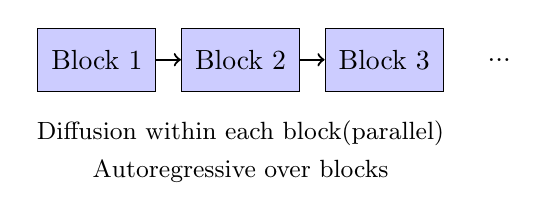
\begin{tikzpicture}[scale=0.73]
                        \node[
                            draw,
                            fill=blue!20,
                            minimum width=1.5cm,
                            minimum height=0.8cm
                        ] (b1) at (0,0) {Block 1};
                        \node[
                            draw,
                            fill=blue!20,
                            minimum width=1.5cm,
                            minimum height=0.8cm
                        ] (b2) at (2.5,0) {Block 2};
                        \node[
                            draw,
                            fill=blue!20,
                            minimum width=1.5cm,
                            minimum height=0.8cm
                        ] (b3) at (5,0) {Block 3};
                        \node (dots) at (7,0) {...};

                        \draw[->, thick] (b1) -- (b2) node[midway, above] {};
                        \draw[->, thick] (b2) -- (b3) node[midway, above] {};

                        \node[below=0.25cm of b2, align=center]
                            {\small Diffusion within each block(parallel)};
                        \node[below=0.75cm of b2, align=center]
                            {\small Autoregressive over blocks};
                    \end{tikzpicture}
                \end{center}
            \end{column}
            \begin{column}{0.4\textwidth}
                \textbf{Parameterization:} Trade-off through block size $L'$:
                \begin{itemize}
                    \item $L' = 1$ → Pure AR

                    \item $L' = L$ → Pure Diffusion %L is inpurt size%
                \end{itemize}
            \end{column}
        \end{columns}
        \vspace{0.4cm}
        \textbf{Technical Contribution:}
        \begin{itemize}
            \item Optimized training and sampling algorithms

            \item Introduced clipped noise schedules for reduced gradient variance
                during training

            \item SoTA PPL among diffusion models + Variable length generation capabilities
        \end{itemize}
    \end{frame}

    \section{Our Results}

    \subsection{Reproduction}

    % ---------------- Reproduction Tables ----------------

    \begin{frame}{AR vs BD3LM with L'=1}
        % ---------- ROW 1 ----------
        \begin{minipage}{\textwidth}
            \begin{minipage}{0.45\textwidth}
                \centering
                \begin{table}
                    \small
                    \centering
                    Test Perplexities for single token generation on LM1B dataset
                    (800 Training Steps)

                    \vspace{0.2cm}
                    \ra{1.2}
                    \setlength{\tabcolsep}{0.2pt}

                    \begin{tabular}{lc}
                        \toprule                                               & PPL ($\downarrow$) \\
                        \midrule $\textbf{Autoregressive}$                     & \textbf{1893}      \\
                        \midrule $\text{\textbf{BD3LM} L'=1}$                  & 2231               \\
                        \midrule $\text{\textbf{BD3LM} L'=1 + Tuned Schedule}$ & 2220               \\
                        \bottomrule
                    \end{tabular}
                \end{table}
            \end{minipage}
            \hfill
            \begin{minipage}{0.47\textwidth}
                \centering
                \includegraphics[width=\linewidth]{fig1.png}

                \small AR
            \end{minipage}
        \end{minipage}

        \vspace{0.5cm}

        % ---------- ROW 2 ----------
        \begin{minipage}{\textwidth}
            \centering
            \begin{minipage}{0.47\textwidth}
                \centering
                \includegraphics[width=\linewidth]{fig2.png}

                \small BD3LM
            \end{minipage}
            \hfill
            \begin{minipage}{0.47\textwidth}
                \centering
                \includegraphics[width=\linewidth]{fig3.png}

                \small BD3LM + Tuned Schedule
            \end{minipage}
        \end{minipage}
    \end{frame}

    \begin{frame}{The Effect of Clipped Noise Schedules}
        \footnotesize

        \begin{columns}[T,onlytextwidth]
            % ----- LEFT: existing table -----
            \begin{column}{0.5\textwidth}
                \begin{table}
                    \centering
                    \small
                    \setlength{\tabcolsep}{6pt}
                    \parbox{1.5\linewidth}{Test Perplexities for single token
                    generation on LM1B dataset\\
                    (400 Pretraining Steps + 100 Fine-tuning Steps) }

                    \vspace{0.2cm}
                    \renewcommand{\arraystretch}{1.1}

                    \begin{tabular}{l l c c}
                        \toprule L'                   & Clipping                & PPL           & Var.\ NELBO    \\
                        \midrule \multirow{2}{*}{128} & $\mathcal{U}[0, 0.5]$   & 1000          & 10.00          \\
                                                      & $\mathcal{U}[0, 1]$     & 1000          & 10.00          \\
                        \midrule \multirow{2}{*}{16}  & $\mathcal{U}[0.3, 0.8]$ & \textbf{1278} & \textbf{10.50} \\
                                                      & $\mathcal{U}[0, 1]$     & 1279          & 10.51          \\
                        \midrule \multirow{2}{*}{4}   & $\mathcal{U}[0.5, 1]$   & \textbf{1226} & \textbf{44.41} \\
                                                      & $\mathcal{U}[0, 1]$     & \textbf{1226} & \textbf{44.41} \\
                        \bottomrule
                    \end{tabular}
                \end{table}
            \end{column}

            % ----- RIGHT: commentary placeholder (same as before) -----
            \begin{column}{0.42\textwidth}
                \vspace{1cm}
                \begin{block}{Commentary (placeholder)}
                    \vspace{0.1cm}
                    \textbf{Key takeaways:}
                    \begin{itemize}
                        \item \emph{???}

                        \item \emph{???}

                        \item \emph{???}
                    \end{itemize}

                    \vspace{0.1cm}
                    \emph{Conclusion...}
                \end{block}
            \end{column}
        \end{columns}
    \end{frame}

    \begin{frame}{BD3LMs vs ARs vs Diffusion Models on LM1B}
        \footnotesize

        \begin{columns}[T,onlytextwidth]
            % ----- LEFT: caption + table -----
            \begin{column}{0.58\textwidth}
                \centering
                \parbox{0.95\linewidth}{\centering
                Test perplexities (PPL; $\downarrow$) of models on LM1B. (400 Pretraining
                Steps + 100 Fine-tuning Steps)}

                \vspace{0.2cm}

                \begin{table}
                    \centering
                    \setlength{\tabcolsep}{22pt} % slightly tighter to leave room for the comment box
                    \renewcommand{\arraystretch}{1.15}
                    \begin{tabular}{@{}l r@{}}
                        \toprule                                                       & \textbf{PPL ($\downarrow$)} \\
                        \midrule \multicolumn{2}{@{}l}{\textbf{Autoregressive}}         \\
                        Transformer                                                    & 3042                        \\
                        \midrule \multicolumn{2}{@{}l}{\textbf{Diffusion}}              \\
                        SEDD                                                           & 1447                        \\
                        MDLM                                                           & 1616                        \\
                        \midrule \multicolumn{2}{@{}l}{\textbf{Block diffusion (Ours)}} \\
                        BD3-LMs $L' = 16$                                              & 1278                        \\
                        \hspace{1.3cm} $L' = 8$                                        & 1734                        \\
                        \hspace{1.3cm} $L' = 4$                                        & \textbf{1226}               \\
                        \bottomrule
                    \end{tabular}
                \end{table}
            \end{column}

            % ----- RIGHT: commentary placeholder -----
            \begin{column}{0.42\textwidth}
                \vspace{0.9cm}
                \begin{block}{Commentary (placeholder)}
                    \vspace{0.1cm}
                    \textbf{Key takeaways:}
                    \begin{itemize}
                        \item \emph{???}

                        \item \emph{???}

                        \item \emph{???}
                    \end{itemize}

                    \vspace{0.1cm}
                    \emph{Conclusion...}
                \end{block}
            \end{column}
        \end{columns}
    \end{frame}

    \begin{frame}{BD3LMs vs ARs vs Diffusion Models on OWT}
        \footnotesize

        \begin{columns}[T,onlytextwidth]
            % ----- LEFT: caption + table -----
            \begin{column}{0.58\textwidth}
                \centering
                \parbox{0.95\linewidth}{\centering
                Test perplexities (PPL; $\downarrow$) of models on OWT. (800 Pretraining
                Steps + 800 Fine-tuning Steps)}

                \vspace{0.2cm}

                \begin{table}
                    \centering
                    \setlength{\tabcolsep}{22pt}
                    \renewcommand{\arraystretch}{1.15}
                    \begin{tabular}{@{}l r@{}}
                        \toprule                                                       & \textbf{PPL ($\downarrow$)} \\
                        \midrule \multicolumn{2}{@{}l}{\textbf{Autoregressive}}         \\
                        Transformer                                                    & 2036                        \\
                        \midrule \multicolumn{2}{@{}l}{\textbf{Diffusion}}              \\
                        SEDD                                                           & $2120$                      \\
                        MDLM                                                           & $2101$                      \\
                        \midrule \multicolumn{2}{@{}l}{\textbf{Block diffusion (Ours)}} \\
                        BD3-LMs $L' = 16$                                              & $1939$                      \\
                        \hspace{1.3cm} $L' = 8$                                        & $1941$                      \\
                        \hspace{1.3cm} $L' = 4$                                        & $\textbf{1935}$             \\
                        \bottomrule
                    \end{tabular}
                \end{table}
            \end{column}

            % ----- RIGHT: commentary placeholder -----
            \begin{column}{0.42\textwidth}
                \vspace{0.9cm}
                \begin{block}{Commentary (placeholder)}
                    \vspace{0.1cm}
                    \textbf{Key takeaways:}
                    \begin{itemize}
                        \item \emph{???}

                        \item \emph{???}

                        \item \emph{???}
                    \end{itemize}

                    \vspace{0.1cm}
                    \emph{Conclusion...}
                \end{block}
            \end{column}
        \end{columns}
    \end{frame}

    \begin{frame}{Performance on other Datasets}
        \centering
        \footnotesize

        \parbox{0.95\linewidth}{\centering}
        {Zero-shot validation perplexities ($\downarrow$) of models trained on OWT.(?training steps?)}

        \vspace{0.25cm}

        \begin{table}
            \centering
            \setlength{\tabcolsep}{15pt}
            \renewcommand{\arraystretch}{1.25}
            \begin{tabular}{@{}lcccc@{}}
                \toprule             & \textbf{LM1B} & \textbf{Lambada} & \textbf{Wikitext} \\
                \midrule \textbf{AR} & 2388          & 1550             & \textbf{2875}     \\
                \midrule SEDD        & 2742          & 1562             & 3335              \\
                MDLM                 & 2722          & 1556             & 3283              \\
                BD3-LM $L' = 4$      & \textbf{2196} & \textbf{1438}    & 3143              \\
                \bottomrule
            \end{tabular}%
        \end{table}

        \vspace{0.25cm}

        \begin{block}{Commentary (placeholder)}
            \textbf{Key takeaways:}
            \begin{itemize}
                \item \emph{??? (e.g., BD3-LM improves on \ldots compared to diffusion
                    baselines)}

                \item \emph{??? (e.g., note where AR is still best / gap remains)}

                \item \emph{??? (e.g., mention that diffusion values are upper bounds
                    if relevant)}
            \end{itemize}
            \emph{Conclusion...}
        \end{block}
    \end{frame}

    \begin{frame}{Variable-Length Sequence Generation}
        \centering
        \footnotesize % shrink the whole slide (matches the style used elsewhere)

        \begin{table}[t]
            \centering
            \caption{\scriptsize Generation length statistics from sampling 10
            documents from models trained on OWT.(?training steps?)}
            \label{tab:gen_length_stats}

            \setlength{\tabcolsep}{4pt} % tighter columns
            \renewcommand{\arraystretch}{1.05} % tighter rows
            \scriptsize % make the table text smaller than the slide default

            \begin{tabular}{lrr}
                \toprule               & \multicolumn{1}{c}{\shortstack{Median\\\# tokens}} & \multicolumn{1}{c}{\shortstack{Max\\\# tokens}} \\
                \midrule OWT train set & 717                                                & 131K                                            \\
                AR                     & 4008                                               & 131K                                            \\
                \midrule SEDD          & 1021                                               & 1024                                            \\
                BD3-LM $L' = 16$       & 798                                                & 2927                                            \\
                \bottomrule
            \end{tabular}
        \end{table}

        \vspace{0.15cm} % slightly smaller gap than before

        \begin{block}{Commentary (placeholder)}
            \scriptsize % shrink the commentary text too
            \textbf{Key takeaways:}
            \begin{itemize}
                \item \emph{??? (e.g., diffusion models are constrained in max length,
                    BD alleviates this)}

                \item \emph{??? (e.g., compare median vs max lengths across AR/SEDD/BD3)}

                \item \emph{??? (e.g., mention practical implication for long-form
                    generation)}
            \end{itemize}
            \emph{Conclusion...}
        \end{block}
    \end{frame}

    \begin{frame}{Sample Quality}
        \centering
        \begin{table}[t]
            \centering
            \caption{Generative Perplexity (Gen.PPL;↓) and number of Function
            Evaluations (NFEs;↓) of 300 samples. All models are trained on OWT.
            (?training steps?)}
            \label{tab:gen_ppl_nfe}
            \begin{tabular}{lrrrr}
                \toprule                                                           & \multicolumn{2}{c}{$L = 1024$} & \multicolumn{2}{c}{$L = 2048$} \\
                \cmidrule(lr){2-3}\cmidrule(lr){4-5} Model                         & Gen.\ PPL                      & NFEs                          & Gen.\ PPL      & NFEs \\
                \midrule AR                                                        & 14.1                           & 1K                            & 13.2           & 2K   \\
                \midrule \addlinespace \multicolumn{5}{l}{\textbf{Diffusion}}       \\
                SEDD                                                               & 52.0                           & 1K                            & --             & --   \\
                MDLM                                                               & 46.8                           & 1K                            & 41.3           & 2K   \\
                \midrule \addlinespace \multicolumn{5}{l}{\textbf{Block Diffusion}} \\
                SSD-LM $L' = 25$                                                   & 37.2                           & 40K                           & 35.3           & 80K  \\
                \addlinespace \hspace{1em}281.3                                    & 1K                             & 281.9                         & 2K              \\ % (όπως φαίνεται στον πίνακα)
                BD3-LMs $L' = 16$                                                  & 32.97                          & 1K                            & 31.42          & 2K   \\
                \hspace{2em}$L' = 8$                                               & 29.35                          & 1K                            & 27.42          & 2K   \\
                \hspace{2em}$L' = 4$                                               & \textbf{24.74}                 & 1K                            & \textbf{23.85} & 2K   \\
                \bottomrule
            \end{tabular}
        \end{table}
    \end{frame}

    \begin{frame}{Effect of Different Noise Schedules}
        \centering
        \scriptsize % smaller than footnotesize to help height fit

        \begin{columns}[T,onlytextwidth]
            % ----- LEFT: existing table -----
            \begin{column}{0.62\textwidth}
                \centering
                \begin{table}[t]
                    \centering
                    \caption{\scriptsize Effect of noise schedule on PPL and
                    variance of NELBO for different $L'$ on LM1B. (?training steps?)}
                    \label{tab:noise_schedule_ablation}

                    \setlength{\tabcolsep}{3pt}
                    \renewcommand{\arraystretch}{0.95}

                    \resizebox{!}{0.36\textheight}{%
                    \begin{tabular}{lcc}
                        \toprule Noise schedule                        & PPL            & Var.\ NELBO   \\
                        \midrule \multicolumn{3}{l}{\textbf{$L' = 4$}}  \\
                        Clipped                                        &                &               \\
                        \hspace{1em}$\mathcal{U}[0.45, 0.95]$          & \textbf{29.21} & \textbf{6.24} \\
                        \hspace{1em}$\mathcal{U}[0.3, 0.8]$            & 29.38          & 10.33         \\
                        Linear $\mathcal{U}[0,1]$                      & 30.18          & 23.45         \\
                        Logarithmic                                    & 30.36          & 23.53         \\
                        Square root                                    & 31.41          & 26.43         \\
                        \midrule \multicolumn{3}{l}{\textbf{$L' = 16$}} \\
                        Clipped                                        &                &               \\
                        \hspace{1em}$\mathcal{U}[0.45, 0.95]$          & 31.42          & 3.60          \\
                        \hspace{1em}$\mathcal{U}[0.3, 0.8]$            & \textbf{31.12} & \textbf{3.58} \\
                        Linear $\mathcal{U}[0,1]$                      & 31.72          & 7.62          \\
                        Square                                         & 31.43          & 13.03         \\
                        Cosine                                         & 31.41          & 13.00         \\
                        \bottomrule
                    \end{tabular}%
                    }
                \end{table}
            \end{column}

            % ----- RIGHT: commentary placeholder (matching earlier slides) -----
            \begin{column}{0.38\textwidth}
                \vspace{0.9cm}
                \begin{block}{Commentary (placeholder)}
                    \vspace{0.1cm}
                    \textbf{Key takeaways:}
                    \begin{itemize}
                        \item \emph{???}

                        \item \emph{???}

                        \item \emph{???}
                    \end{itemize}

                    \vspace{0.1cm}
                    \emph{Conclusion...}
                \end{block}
            \end{column}
        \end{columns}
    \end{frame}

    \subsection{Extensions}

    \begin{frame}{Noise Scheduling in Masked Diffusion (Summary)}
        \small \textbf{Continuous time index:}
        \[
            t \sim \mathcal{U}[0,1]
        \]

        \vspace{0.15cm}
        \textbf{Noise schedule $\Rightarrow$ masked probability:}
        \[
            \begin{aligned}
                p(t) & :\ \text{masked probability induced by the noise schedule}
            \end{aligned}
        \]

        \vspace{0.1cm}
        \textbf{Keep (no-mask) probability:}
        \[
            a(t) = 1 - p(t)
        \]

        \vspace{0.08cm}
        \textbf{Loss scaling induced by the schedule:}
        \[
            \text{loss scaling}(t) \;=\; \frac{a'(t)}{1-a(t)}
        \]

        % \vspace{0.01cm}
        \begin{block}{Intuition}
            The noise schedule sets \emph{where} the model learns via $p(t)$ (masking
            rate). When sampling $t \sim \mathcal{U}[0,1]$,
            $\text{loss\_scaling}(t)=\frac{a'(t)}{1-a(t)}$ acts as a weight on
            the per-token log-likelihood term so the discrete estimator matches
            the continuous-time integral/ELBO and balances low- vs high-noise regions.
        \end{block}
    \end{frame}

    \begin{frame}{Already Implemented Noise Schedules}
        \footnotesize
        \centering
        \setlength{\tabcolsep}{9pt}
        \renewcommand{\arraystretch}{2.9}

        \begin{table}
            \centering
            \begin{tabular}{@{}l l l@{}}
                \toprule \textbf{Schedule} & \textbf{$p(t)$}                                        & \textbf{$\text{loss\_scaling}(t)$}                                                                                                          \\
                \midrule LogLinear         & $t$                                                    & $-\dfrac{1}{t}$                                                                                                                             \\
                Square                     & $t^{2}$                                                & $-\dfrac{2}{t}$                                                                                                                             \\
                Square root                & $t^{0.5}$                                              & $-\dfrac{1}{2t}$                                                                                                                            \\
                Logarithmic                & $\dfrac{\log(1+t)}{\log 2}$                            & $-\dfrac{1}{(1+t)\,\log(1+t)}$                                                                                                              \\
                Cosine                     & $1-(1-\varepsilon)\cos\!\left(\dfrac{\pi t}{2}\right)$ & $-\dfrac{\left(\frac{\pi}{2}\right)(1-\varepsilon)\sin\!\left(\frac{\pi t}{2}\right)}{1-(1-\varepsilon)\cos\!\left(\frac{\pi t}{2}\right)}$ \\
                \bottomrule
            \end{tabular}
        \end{table}
    \end{frame}

    \begin{frame}{Gaussian \& Bimodal Gaussian Noise Schedules}
        \scriptsize \textbf{Goal:} sample a masked probability $p(t)\in(0,1)$
        from $t\sim\mathcal{U}[0,1]$.

        \vspace{0.08cm}
        \textbf{Gaussian schedule (truncated to $(0,1)$):}\\
        Let $\alpha=\frac{0-\mu}{\sigma}$, $\beta=\frac{1-\mu}{\sigma}$,
        $\Phi_{\alpha}=\Phi(\alpha)$, $\Phi_{\beta}=\Phi(\beta)$. For
        $t\in(0,1)$:
        \[
            z(t)=\Phi^{-1}\!\big(\Phi_{\alpha}+ t(\Phi_{\beta}-\Phi_{\alpha})\big
            ), \qquad p(t)=\mu+\sigma z(t)\in(0,1).
        \]
        With $Z=\Phi_{\beta}-\Phi_{\alpha}$ and $\varphi(\cdot)$ the standard normal
        pdf:
        \[
            \text{loss\_scaling}(t)=\frac{a'(t)}{1-a(t)}=-\frac{p'(t)}{p(t)}=-\frac{\sigma
            Z}{\varphi(z(t))\,p(t)}.
        \]

        \vspace{0.05cm}
        \textbf{Bimodal Gaussian schedule (mixture):}\\
        Choose a split weight $w\in(0,1)$ (denote $w_{1}=w$, $w_{2}=1-w$). With probability
        $w$ use $(\mu_{1},\sigma_{1})$, otherwise use $(\mu_{2},\sigma_{2})$:
        \[
            t_{1}=\frac{t}{w_{1}}\;\; (t<w_{1}), \qquad t_{2}=\frac{t-w_{1}}{w_{2}}
            \;\; (t\ge w_{1}), \qquad p(t)=
            \begin{cases}
                \mu_{1}+\sigma_{1}z_{1}(t_{1}), & t<w_{1}    \\
                \mu_{2}+\sigma_{2}z_{2}(t_{2}), & t\ge w_{1}
            \end{cases}
        \]
        where each $z_{i}(\cdot)$ is defined as above (with its own
        $\alpha_{i},\beta_{i},\Phi_{\alpha_i},\Phi_{\beta_i}$ and $Z_{i}$). The
        resulting scaling is piecewise:
        \[
            \text{loss\_scaling}(t)= -\frac{1}{p(t)}
            \begin{cases}
                \frac{1}{w_1}\frac{\sigma_1 Z_1}{\varphi(z_1(t_1))}, & t<w_{1}    \\[2pt]
                \frac{1}{w_2}\frac{\sigma_2 Z_2}{\varphi(z_2(t_2))}, & t\ge w_{1}
            \end{cases}
        \]
    \end{frame}

    \begin{frame}{Exploring New Schedules}
        \begin{itemize}
            \item Motivation for designing alternative noise schedules

            \item Trade-off between stability and generation quality

            \item Impact on gradient variance

            \item Compatibility with block diffusion framework
        \end{itemize}
    \end{frame}

    \begin{frame}{New Schedules' Results}
        \tiny
        \centering
        \vspace{-0.3em}
        % \textbf{Perplexities (PPL) and Var.\ NELBO for implemented vs new schedules}\par
        \vspace{0.4em}

        \begin{table}
            \caption{Perplexities (PPL) and Var.\ NELBO for implemented vs new schedules
            on LM1B (400 Pretraining Steps + 100 Fine-tuning Steps). B.G. stands for Bimodal Gaussian}
            \centering
            \setlength{\tabcolsep}{2.0pt} % was 2.2pt (slightly tighter to fit extra rows)
            \renewcommand{\arraystretch}{0.90} % was 0.95

            \resizebox{\textwidth}{!}{%
            \begin{tabular}{c l c c | l c c}
                \toprule \multirow{2}{*}{Block Size} & \multicolumn{3}{c|}{\textbf{Already Implemented}} & \multicolumn{3}{c}{\textbf{Newly Implemented}} \\
                \cmidrule(lr){2-4}\cmidrule(lr){5-7} & Noise Schedule                                    & PPL                                           & Var.\ NELBO & Noise Schedule   & PPL  & Var.\ NELBO \\
                \midrule

\multirow{4}{*}{128}       & Loglinear                                                                   & 1000                                          & 10.00       & Gaussian ($\mu=$0.5)           & 1000 & 10.00       \\
                                                     & Loglinear $\mathcal{U}[0,\,0.5]$                  & 1000                                          & 10.00       & Gaussian ($\mu=$0.6)           & 1000 & 10.00       \\
                                                     & Cosine                                            & 1000                                          & 10.00       & B.G. ($\mu_1=0.3, w_1=0.6$)    & 1000 & 10.00       \\
                                                     & Cosine $\mathcal{U}[0,\,0.5]$                     & 1000                                          & 10.00       & B.G. ($\mu_1=0.1, w_1=0.6$)    & 1000 & 10.00       \\
                \midrule

\multirow{4}{*}{16}        & Loglinear                                                                   & 1279                                          & 10.50       & Gaussian ($\mu=$0.5)           & 1234 & 10.00       \\
                                                     & Loglinear $\mathcal{U}[0.3,\,0.8]$                & 1278                                          & 10.51       & Gaussian ($\mu=$0.6)           & 1235 & 10.00       \\
                                                     & Cosine                                            & 1236                                          & 10.00       & B.G. ($\mu_1=0.3, w_1=0.6$)    & 1254 & 10.00       \\
                                                     & Cosine $\mathcal{U}[0.3,\,0.8]$                   & 1235                                          & 10.00       & B.G. ($\mu_1=0.1, w_1=0.6$)    & 1295 & 10.00       \\
                \midrule

\multirow{4}{*}{4}         & Loglinear                                                                   & 1226                                          & 44.41       & Gaussian ($\mu=$0.5)           & 1000 & 10.00       \\
                                                     & Loglinear $\mathcal{U}[0.5,\,1]$                  & 1226                                          & 44.41       & Gaussian ($\mu=$0.6)           & 1000 & 10.00       \\
                                                     & Cosine                                            & 1000                                          & 10.00       & B.G. ($\mu_1=0.3, w_1=0.6$)    & 1000 & 10.00       \\
                                                     & Cosine $\mathcal{U}[0.5,\,1]$                     & 1000                                          & 10.00       & B.G. ($\mu_1=0.1, w_1=0.6$)    & 1000 & 10.00       \\
                \bottomrule
            \end{tabular}%
            }
        \end{table}
        \vspace{-0.6em}
    \end{frame}

    \begin{frame}{Reweighted Losses for Improved Diffusion Objective}
        \begin{figure}
            \centering
            \includegraphics[width=\linewidth]{reweighting.png}
        \end{figure}
    \end{frame}

    \begin{frame}{Reweighted Losses for Masked Diffusion}
        \begin{itemize}
            \item Initial Reweighted NELBO:
                \[
                    \cL^{\tilde{w}}(\bx) = -\int_{0}^{1}\textcolor{red}{\tilde{w}(\textcolor{black}{t})
                    }\frac{\alpha_{t}'}{1 - \alpha_{t}}\E_{q(\bz_t|\bx)}\left[\delta
                    _{\bz_t, m}\cdot \bx^{\top}\log \mu_{\theta}(\bz_{t})\right]
                    \diff t
                \]

            \item Reparameterization trick:
                $\lambda(t) = \log \frac{\alpha_{t}}{1 - \alpha_{t}}$:
                \[
                    \cL^{\hat{w}}(\bx) = -\int_{0}^{1}\textcolor{blue}{\hat{w}(\textcolor{black}{\lambda(t)})
                    }\frac{\alpha_{t}'}{1 - \alpha_{t}}\E_{q(\bz_t|\bx)}\left[\delta
                    _{\bz_t, m}\cdot \bx^{\top}\log \mu_{\theta}(\bz_{t})\right]
                    \diff t
                \]
        \end{itemize}
        \begin{table}[t]
            \centering
            % \caption{Weighting functions investigated for masked diffusion models. All functions, excluding the simple weighting, were migrated from continuous diffusion weightings by matching $\hat{w}(\lambda)$. Note that only the sigmoid, flow matching (FM), and simple weightings satisfy the necessary monotonicity requirement when paired with the cosine schedule $\alpha_t = 1 - \cos(\frac{\pi}{2}(1 - t))$.}
            % \vskip 0.1in
            \footnotesize
            \begin{tabular}{lcccc}
                \toprule Name & $\lambda(t)$                                              & $\hat{w}(\lambda)$                                                          & $\tilde{w}(t)$                                    \\
                \midrule EDM  & \multirow{5}{*}{$\log \frac{\alpha_{t}}{1 - \alpha_{t}}$} & $p_{\mathcal{N}(2.4, 2.4^2)}(\lambda)\frac{e^{-\lambda}+ 0.5^{2}}{0.5^{2}}$ & $w(\lambda(t))$                                   \\
                [4pt] IDDPM   &                                                           & $\mathrm{sech}(\frac{\lambda}{2})$                                          & $2\sqrt{\alpha_{t}(1 - \alpha_{t})}$              \\
                [4pt] Sigmoid &                                                           & $\mathrm{sigmoid}(-\lambda + k)$                                            & $\frac{1-\alpha_{t}}{1 - (1 - e^{-k})\alpha_{t}}$ \\
                [4pt] FM      &                                                           & $e^{-\frac{\lambda}{2}}$                                                    & $\sqrt{\frac{1 - \alpha_{t}}{\alpha_{t}}}$        \\
                [4pt] Simple  &                                                           & -                                                                           & $-\frac{1 - \alpha_{t}}{\alpha_{t}'}$             \\
                \bottomrule
            \end{tabular}
        \end{table}
    \end{frame}

    \begin{frame}{Reweighted Losses Results}
        \begin{table}
            \small
            \centering
            Extended Table 3: Test Perplexities

            \vspace{0.2cm}
            \ra{1.2}
            \setlength{\tabcolsep}{2pt}

            \begin{tabular}{lcccccc}
                \toprule                                            & PPL ($\downarrow$) \\
                \midrule \multicolumn{2}{l}{\textbf{Autoregressive}} \\
                $\text{Transformer}$                                & 1221               \\
                \midrule \multicolumn{2}{l}{\textbf{Diffusion}}      \\
                SEDD                                                & 1403               \\
                MDLM                                                & 1370               \\
                \midrule                                             % UPDATED LINE BELOW
                \textbf{Block diffusion}                            & \textbf{Base}     & \textbf{IDDPM} & \textbf{EDM} & \makecell{\textbf{Sigmoid} \\ \textbf{(k = 0)}} & \textbf{FM} & \textbf{Simple} \\
                BD3-LMs $L'=16$                                     & 1345              & 252            & 49.88        & 36.06                                           & 76213       & 53070           \\
                \hspace{4.1em} $L'=8$                               & 1210              & 249            & 49.14        & 35.79                                           & 109169      & 36010741760     \\
                \hspace{4.1em} $L'=4$                               & 1176              & 246            & 49.01        & \textbf{35.08}                                  & 67332       & 2396260         \\
                \bottomrule
            \end{tabular}
        \end{table}
    \end{frame}

    \section{Conclusion \& Future Work}

    \section{Team Organization}

    \section{Retrospection}
\end{document}